
%% bare_conf.tex
%% V1.4b
%% 2015/08/26
%% by Michael Shell
%% See:
%% http://www.michaelshell.org/
%% for current contact information.
%%
%% This is a skeleton file demonstrating the use of IEEEtran.cls
%% (requires IEEEtran.cls version 1.8b or later) with an IEEE
%% conference paper.
%%
%% Support sites:
%% http://www.michaelshell.org/tex/ieeetran/
%% http://www.ctan.org/pkg/ieeetran
%% and
%% http://www.ieee.org/

%%*************************************************************************


% *** Authors should verify (and, if needed, correct) their LaTeX system  ***
% *** with the testflow diagnostic prior to trusting their LaTeX platform ***
% *** with production work. The IEEE's font choices and paper sizes can   ***
% *** trigger bugs that do not appear when using other class files.       ***                          ***
% The testflow support page is at:
% http://www.michaelshell.org/tex/testflow/



\documentclass[conference]{IEEEtran}
% Some Computer Society conferences also require the compsoc mode option,
% but others use the standard conference format.
%
% If IEEEtran.cls has not been installed into the LaTeX system files,
% manually specify the path to it like:
% \documentclass[conference]{../sty/IEEEtran}





% Some very useful LaTeX packages include:
% (uncomment the ones you want to load)


% *** MISC UTILITY PACKAGES ***
%
%\usepackage{ifpdf}
% Heiko Oberdiek's ifpdf.sty is very useful if you need conditional
% compilation based on whether the output is pdf or dvi.
% usage:
% \ifpdf
%   % pdf code
% \else
%   % dvi code
% \fi
% The latest version of ifpdf.sty can be obtained from:
% http://www.ctan.org/pkg/ifpdf
% Also, note that IEEEtran.cls V1.7 and later provides a builtin
% \ifCLASSINFOpdf conditional that works the same way.
% When switching from latex to pdflatex and vice-versa, the compiler may
% have to be run twice to clear warning/error messages.






% *** CITATION PACKAGES ***
%
\usepackage{cite}
% cite.sty was written by Donald Arseneau
% V1.6 and later of IEEEtran pre-defines the format of the cite.sty package
% \cite{} output to follow that of the IEEE. Loading the cite package will
% result in citation numbers being automatically sorted and properly
% "compressed/ranged". e.g., [1], [9], [2], [7], [5], [6] without using
% cite.sty will become [1], [2], [5]--[7], [9] using cite.sty. cite.sty's
% \cite will automatically add leading space, if needed. Use cite.sty's
% noadjust option (cite.sty V3.8 and later) if you want to turn this off
% such as if a citation ever needs to be enclosed in parenthesis.
% cite.sty is already installed on most LaTeX systems. Be sure and use
% version 5.0 (2009-03-20) and later if using hyperref.sty.
% The latest version can be obtained at:
% http://www.ctan.org/pkg/cite
% The documentation is contained in the cite.sty file itself.






% *** GRAPHICS RELATED PACKAGES ***
%
\ifCLASSINFOpdf
  % \usepackage[pdftex]{graphicx}
  % declare the path(s) where your graphic files are
  % \graphicspath{{../pdf/}{../jpeg/}}
  % and their extensions so you won't have to specify these with
  % every instance of \includegraphics
  % \DeclareGraphicsExtensions{.pdf,.jpeg,.png}
\else
  % or other class option (dvipsone, dvipdf, if not using dvips). graphicx
  % will default to the driver specified in the system graphics.cfg if no
  % driver is specified.
  % \usepackage[dvips]{graphicx}
  % declare the path(s) where your graphic files are
  % \graphicspath{{../eps/}}
  % and their extensions so you won't have to specify these with
  % every instance of \includegraphics
  % \DeclareGraphicsExtensions{.eps}
\fi
% graphicx was written by David Carlisle and Sebastian Rahtz. It is
% required if you want graphics, photos, etc. graphicx.sty is already
% installed on most LaTeX systems. The latest version and documentation
% can be obtained at: 
% http://www.ctan.org/pkg/graphicx
% Another good source of documentation is "Using Imported Graphics in
% LaTeX2e" by Keith Reckdahl which can be found at:
% http://www.ctan.org/pkg/epslatex
%
% latex, and pdflatex in dvi mode, support graphics in encapsulated
% postscript (.eps) format. pdflatex in pdf mode supports graphics
% in .pdf, .jpeg, .png and .mps (metapost) formats. Users should ensure
% that all non-photo figures use a vector format (.eps, .pdf, .mps) and
% not a bitmapped formats (.jpeg, .png). The IEEE frowns on bitmapped formats
% which can result in "jaggedy"/blurry rendering of lines and letters as
% well as large increases in file sizes.
%
% You can find documentation about the pdfTeX application at:
% http://www.tug.org/applications/pdftex
\usepackage{graphicx}
\usepackage{caption}
\usepackage{subcaption}
\graphicspath{{./images/}}
\usepackage{float}
\usepackage{scrextend}
\usepackage{url}

\usepackage{booktabs}
%\usepackage{hyperref}



% *** MATH PACKAGES ***
%
%\usepackage{amsmath}
% A popular package from the American Mathematical Society that provides
% many useful and powerful commands for dealing with mathematics.
%
% Note that the amsmath package sets \interdisplaylinepenalty to 10000
% thus preventing page breaks from occurring within multiline equations. Use:
%\interdisplaylinepenalty=2500
% after loading amsmath to restore such page breaks as IEEEtran.cls normally
% does. amsmath.sty is already installed on most LaTeX systems. The latest
% version and documentation can be obtained at:
% http://www.ctan.org/pkg/amsmath





% *** SPECIALIZED LIST PACKAGES ***
%
%\usepackage{algorithmic}
% algorithmic.sty was written by Peter Williams and Rogerio Brito.
% This package provides an algorithmic environment fo describing algorithms.
% You can use the algorithmic environment in-text or within a figure
% environment to provide for a floating algorithm. Do NOT use the algorithm
% floating environment provided by algorithm.sty (by the same authors) or
% algorithm2e.sty (by Christophe Fiorio) as the IEEE does not use dedicated
% algorithm float types and packages that provide these will not provide
% correct IEEE style captions. The latest version and documentation of
% algorithmic.sty can be obtained at:
% http://www.ctan.org/pkg/algorithms
% Also of interest may be the (relatively newer and more customizable)
% algorithmicx.sty package by Szasz Janos:
% http://www.ctan.org/pkg/algorithmicx




% *** ALIGNMENT PACKAGES ***
%
%\usepackage{array}
% Frank Mittelbach's and David Carlisle's array.sty patches and improves
% the standard LaTeX2e array and tabular environments to provide better
% appearance and additional user controls. As the default LaTeX2e table
% generation code is lacking to the point of almost being broken with
% respect to the quality of the end results, all users are strongly
% advised to use an enhanced (at the very least that provided by array.sty)
% set of table tools. array.sty is already installed on most systems. The
% latest version and documentation can be obtained at:
% http://www.ctan.org/pkg/array


% IEEEtran contains the IEEEeqnarray family of commands that can be used to
% generate multiline equations as well as matrices, tables, etc., of high
% quality.




% *** SUBFIGURE PACKAGES ***
%\ifCLASSOPTIONcompsoc
%  \usepackage[caption=false,font=normalsize,labelfont=sf,textfont=sf]{subfig}
%\else
%  \usepackage[caption=false,font=footnotesize]{subfig}
%\fi
% subfig.sty, written by Steven Douglas Cochran, is the modern replacement
% for subfigure.sty, the latter of which is no longer maintained and is
% incompatible with some LaTeX packages including fixltx2e. However,
% subfig.sty requires and automatically loads Axel Sommerfeldt's caption.sty
% which will override IEEEtran.cls' handling of captions and this will result
% in non-IEEE style figure/table captions. To prevent this problem, be sure
% and invoke subfig.sty's "caption=false" package option (available since
% subfig.sty version 1.3, 2005/06/28) as this is will preserve IEEEtran.cls
% handling of captions.
% Note that the Computer Society format requires a larger sans serif font
% than the serif footnote size font used in traditional IEEE formatting
% and thus the need to invoke different subfig.sty package options depending
% on whether compsoc mode has been enabled.
%
% The latest version and documentation of subfig.sty can be obtained at:
% http://www.ctan.org/pkg/subfig




% *** FLOAT PACKAGES ***
%
%\usepackage{fixltx2e}
% fixltx2e, the successor to the earlier fix2col.sty, was written by
% Frank Mittelbach and David Carlisle. This package corrects a few problems
% in the LaTeX2e kernel, the most notable of which is that in current
% LaTeX2e releases, the ordering of single and double column floats is not
% guaranteed to be preserved. Thus, an unpatched LaTeX2e can allow a
% single column figure to be placed prior to an earlier double column
% figure.
% Be aware that LaTeX2e kernels dated 2015 and later have fixltx2e.sty's
% corrections already built into the system in which case a warning will
% be issued if an attempt is made to load fixltx2e.sty as it is no longer
% needed.
% The latest version and documentation can be found at:
% http://www.ctan.org/pkg/fixltx2e


%\usepackage{stfloats}
% stfloats.sty was written by Sigitas Tolusis. This package gives LaTeX2e
% the ability to do double column floats at the bottom of the page as well
% as the top. (e.g., "\begin{figure*}[!b]" is not normally possible in
% LaTeX2e). It also provides a command:
%\fnbelowfloat
% to enable the placement of footnotes below bottom floats (the standard
% LaTeX2e kernel puts them above bottom floats). This is an invasive package
% which rewrites many portions of the LaTeX2e float routines. It may not work
% with other packages that modify the LaTeX2e float routines. The latest
% version and documentation can be obtained at:
% http://www.ctan.org/pkg/stfloats
% Do not use the stfloats baselinefloat ability as the IEEE does not allow
% \baselineskip to stretch. Authors submitting work to the IEEE should note
% that the IEEE rarely uses double column equations and that authors should try
% to avoid such use. Do not be tempted to use the cuted.sty or midfloat.sty
% packages (also by Sigitas Tolusis) as the IEEE does not format its papers in
% such ways.
% Do not attempt to use stfloats with fixltx2e as they are incompatible.
% Instead, use Morten Hogholm'a dblfloatfix which combines the features
% of both fixltx2e and stfloats:
%
% \usepackage{dblfloatfix}
% The latest version can be found at:
% http://www.ctan.org/pkg/dblfloatfix




% *** PDF, URL AND HYPERLINK PACKAGES ***
%
%\usepackage{url}
% url.sty was written by Donald Arseneau. It provides better support for
% handling and breaking URLs. url.sty is already installed on most LaTeX
% systems. The latest version and documentation can be obtained at:
% http://www.ctan.org/pkg/url
% Basically, \url{my_url_here}.




% *** Do not adjust lengths that control margins, column widths, etc. ***
% *** Do not use packages that alter fonts (such as pslatex).         ***
% There should be no need to do such things with IEEEtran.cls V1.6 and later.
% (Unless specifically asked to do so by the journal or conference you plan
% to submit to, of course. )


% correct bad hyphenation here
\hyphenation{op-tical net-works semi-conduc-tor}


\begin{document}
%
% paper title
% Titles are generally capitalized except for words such as a, an, and, as,
% at, but, by, for, in, nor, of, on, or, the, to and up, which are usually
% not capitalized unless they are the first or last word of the title.
% Linebreaks \\ can be used within to get better formatting as desired.
% Do not put math or special symbols in the title.
\title{Flexible Computer Assisted Transcription of Historical Documents Through Subword Spotting}


% author names and affiliations
% use a multiple column layout for up to three different
% affiliations
\author{\IEEEauthorblockN{Brian Davis, Robert Clawson and William Barrett}
\IEEEauthorblockA{Department of Computer Science, Brigham Young University\\
Provo, Utah\\
Email: briandavis@byu.net}
%\and
%\IEEEauthorblockN{Homer Simpson}
%\IEEEauthorblockA{Twentieth Century Fox\\
%Springfield, USA\\
%Email: homer@thesimpsons.com}
}

% conference papers do not typically use \thanks and this command
% is locked out in conference mode. If really needed, such as for
% the acknowledgment of grants, issue a \IEEEoverridecommandlockouts
% after \documentclass

% for over three affiliations, or if they all won't fit within the width
% of the page, use this alternative format:
% 
%\author{\IEEEauthorblockN{Michael Shell\IEEEauthorrefmark{1},
%Homer Simpson\IEEEauthorrefmark{2},
%James Kirk\IEEEauthorrefmark{3}, 
%Montgomery Scott\IEEEauthorrefmark{3} and
%Eldon Tyrell\IEEEauthorrefmark{4}}
%\IEEEauthorblockA{\IEEEauthorrefmark{1}School of Electrical and Computer Engineering\\
%Georgia Institute of Technology,
%Atlanta, Georgia 30332--0250\\ Email: see http://www.michaelshell.org/contact.html}
%\IEEEauthorblockA{\IEEEauthorrefmark{2}Twentieth Century Fox, Springfield, USA\\
%Email: homer@thesimpsons.com}
%\IEEEauthorblockA{\IEEEauthorrefmark{3}Starfleet Academy, San Francisco, California 96678-2391\\
%Telephone: (800) 555--1212, Fax: (888) 555--1212}
%\IEEEauthorblockA{\IEEEauthorrefmark{4}Tyrell Inc., 123 Replicant Street, Los Angeles, California 90210--4321}}




% use for special paper notices
%\IEEEspecialpapernotice{(Invited Paper)}




% make the title area
\maketitle

% As a general rule, do not put math, special symbols or citations
% in the abstract
%\begin{abstract}
%In the absence of accurate handwriting recognition for historical documents, computer assisted transcription (CAT) methods move into the spotlight. We explore some of the weaknesses of current CAT systems and propose a CAT system, which relies on subword spotting, that overcomes most of these.
%\end{abstract}

%  keywords: CAT, computer assisted transcription, transcription, handwriting, word spotting, character n-gram, subword




% For peer review papers, you can put extra information on the cover
% page as needed:
% \ifCLASSOPTIONpeerreview
% \begin{center} \bfseries EDICS Category: 3-BBND \end{center}
% \fi
%
% For peerreview papers, this IEEEtran command inserts a page break and
% creates the second title. It will be ignored for other modes.
\IEEEpeerreviewmaketitle



%\section{Abstract} %and prior work
Accurate transcription of important historical documents is a costly process, requiring many man-hours. Current handwriting recognition technology does not allow fully automated solutions; during a recent competition for handwriting recognition on historical documents, the top method had a word error rate above 25\%\cite{icdarComp2015}.  However, computer assisted transcription (CAT) methods offer a middle ground between manual and fully automated transcription. CAT methods aim to harness handwriting recognition technology and human efforts together in an effective way. We will explore a few prior CAT systems to examine the state of the art methods. Additionally, crowdsourcing has been a popular means of transcribing large corpi of handwritten documents (e.g. FamilySearch Indexing). We will propose a CAT system which is directed at crowdsourced work, and is particularly adaptable to mobile users.

Toselli, et al\cite{Toselli2010}\footnote{You can find a demo of their system at \url{http://cat.prhlt.upv.es/iht/}} have explored the realm of CAT using the idea of user-verified prefixes. They use a fairly standard HMM recognition model as the backbone of their approach. The recognition is done for a line of text and the user corrects the first error. Recognition is run again reusing the computation up to that point and the correction. Their approach relies on a language model, which means this approach cannot be used to effectively transcribe documents containing non-sentence writing, such as tables and lists. Serrano, et al also have pursued a similar approach, where the user corrects the $n$ words the recognition model had the least confidence in\cite{Serrano2014}.

Robert Clawson designed Intelligent Indexing\cite{Clawson2014}\footnote{You can view a short demo of his system at \url{http://tiny.cc/intelind}}, a CAT system for handwritten documents. Intelligent Indexing relies on finding matching word images in a document and assigning them the same user-specified label.
%, as seen in Fig.~\ref{fig:ii}.
The user oversight of matches was accomplished by showing the user a list of matches (with an adjustable threshold for sensitivity) from which the user removed the false-positive matches. This leveraged the human user's natural ability to discriminate. Zagoris et al\cite{Zagoris2015}\footnote{You can find a demo of their system at \url{http://vc.ee.duth.gr/ws/}} also propose a CAT system which uses word spotting. Rather than focusing on having a user remove bad spots, as the user confirms correct spottings, a relevance feedback loop helps select better results from the word spotting. Both of these approaches allow a few user actions to transcribe many words. However, both of these approaches are limited as they require frequent word repetition to be effective. There are some commonly repeating words for certain documents, but there are many words which repeat infrequently, or not at all, in documents.


%\begin{figure}
%    \centering
%    \begin{subfigure}[t]{0.23\textwidth}
%    		\centering
%    		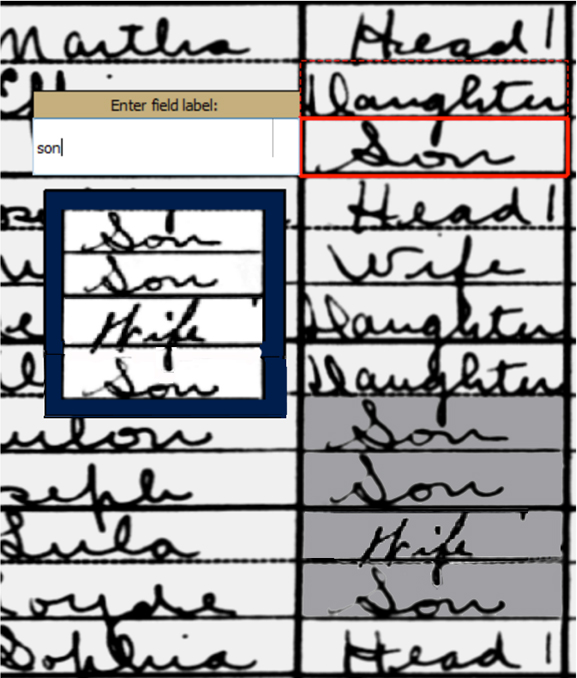
\includegraphics[width=\textwidth]{ii_ex_new_a}
%    		\caption{A small window shows matching words from the column. The user can get rid of bad matches (e.g. ``Wife'') by clicking on them.}
%    	\end{subfigure}
%    	~
%    	\begin{subfigure}[t]{0.23\textwidth}
%    		\centering
%    		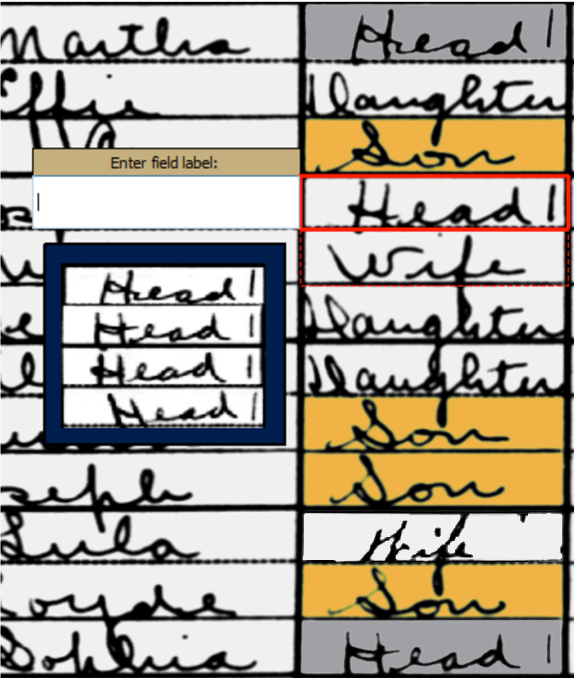
\includegraphics[width=\textwidth]{ii_ex_new_b}
%    		\caption{The matched words are given the same label, indicated by the highlighting, and the red box is advanced to the next word to be transcribed.}
%    	\end{subfigure}
%    	\caption{An example of Clawson's Intelligent Indexing, a CAT system for tabular documents.}
%    	\label{fig:ii}
%\end{figure}

Neudecker and Tzadok\cite{Neudecker2010} presented a CAT system for historical printed documents which is very similar to the CAT system we are presenting here. Their system first segments the individual characters of the documents and runs an OCR engine on them. Those characters with low confidence are then presented to a user for verification in a character session. A single character session contains all the low-confidence character images classified to a single character; the user merely needs to select the incorrect classifications.
An example of their system's character session for the character ``?'' is given in Fig.~\ref{fig:carpet}. 
Then in a word session, a word image is shown to the user with possible transcriptions for the word, from which they select the correct one.

\begin{figure}
    \centering
    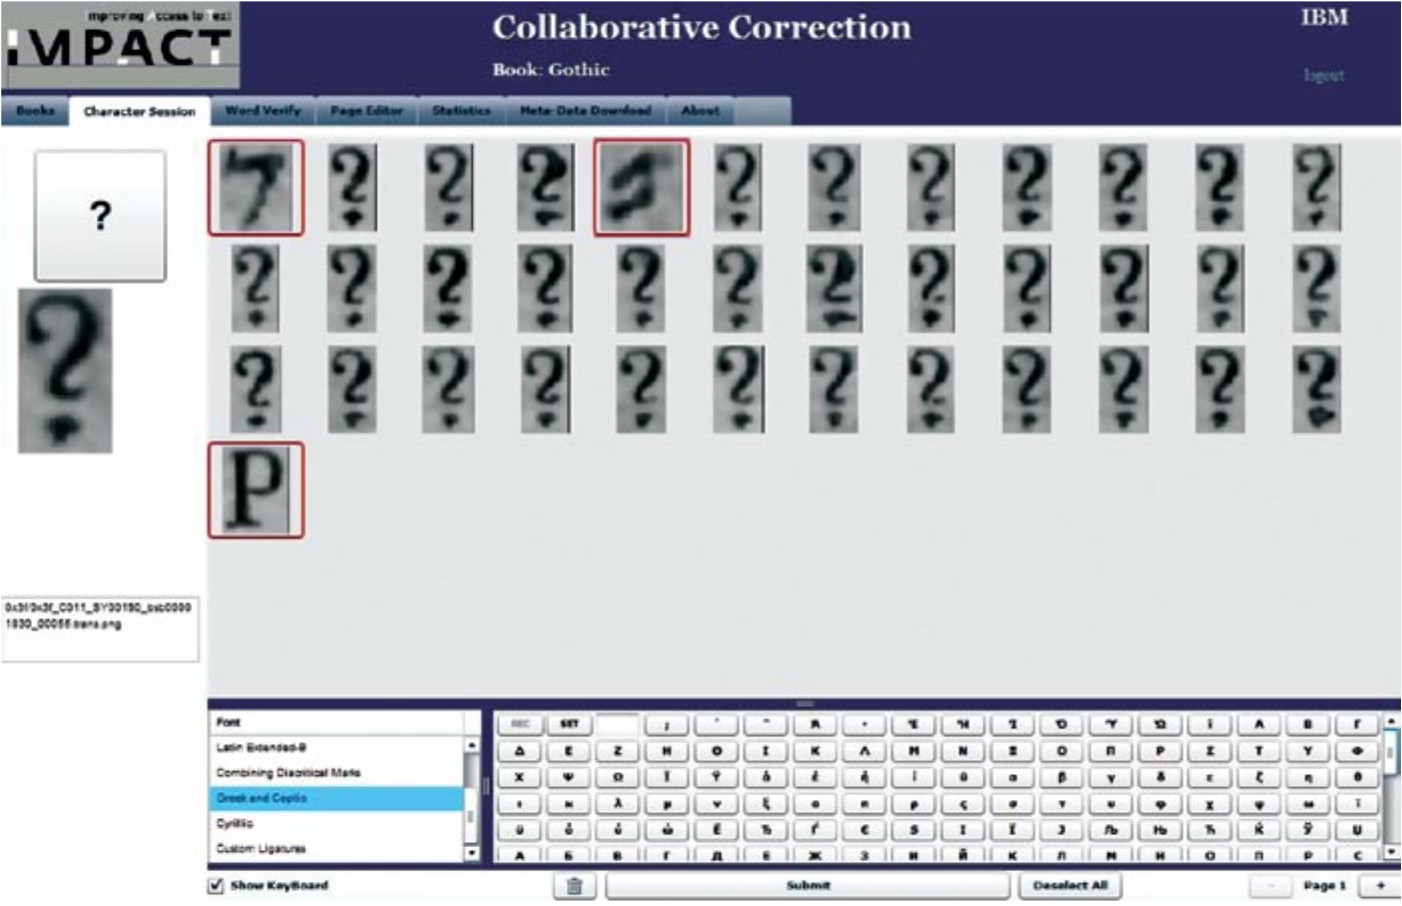
\includegraphics[width=.47\textwidth]{carpet}
    \caption{Screen shot of character session for ``?'' from Neudecker and Tzadok's CAT system, taken directly from their report \cite{Neudecker2010}. Both this method and Intelligent Indexing use an interface that makes it easy for users to simply click on erroneous classifications.}
    \label{fig:carpet}
\end{figure}

There are three key strengths of the system presented in \cite{Neudecker2010}. One is that as long as a documents' characters can be segmented, it can work with that document. The second is that it formats all user tasks as selections, rather than typing, thereby minimizing the time to complete each task and reducing human errors from typing. This also creates a much more enjoyable experience for the user and could be easily adapted to a small touch screen. The third key strength is that it is highly parallelizable for crowd-sourced transcribing. This parallelism is achieved as all character sessions are independent of one another and all word sessions are independent of one another. Our CAT system for handwritten documents will follow this system's flexibility for document types, simple user tasks and parallelizable framework.



Clawson\cite{Clawson2014} and Zagoris et al\cite{Zagoris2015} rely on word spotting to transcribe, which is dependent on frequent word repetition. Neudecker, Tzadok\cite{Neudecker2010} relies on OCR to transcribe, which is dependent on character segmentation, a difficult problem for handwriting.
A happy median, to word spotting and OCR, is character n-gram spotting, which is spotting short subwords (bi- and trigrams) in the words of the document. N-grams have more frequent repetition than words do, but are large enough to spot (i.e. it doesn't require character segmentation). This will provide the backbone of the CAT system we are proposing.

Our system would follow a similar pattern as \cite{Neudecker2010}. N-grams are spotted in the document images. Low confidence spottings are then presented to users to verify (discarding/ignoring incorrect spottings). From the spotted n-grams we are able to generate partial transcriptions of words (we know some, but not all of the letters), from which we can narrow the list of possible transcriptions considerably. Once this list has been narrowed down to a few words (from one or more n-grams being spotted in the word image), this list is presented to a user to select the correct transcription. Fig.~\ref{fig:system_diagram} shows this process. Additionally, spotted n-grams and transcribed word images provide information we can learn from to improve later spotting iterations.

\begin{figure}
    \centering
    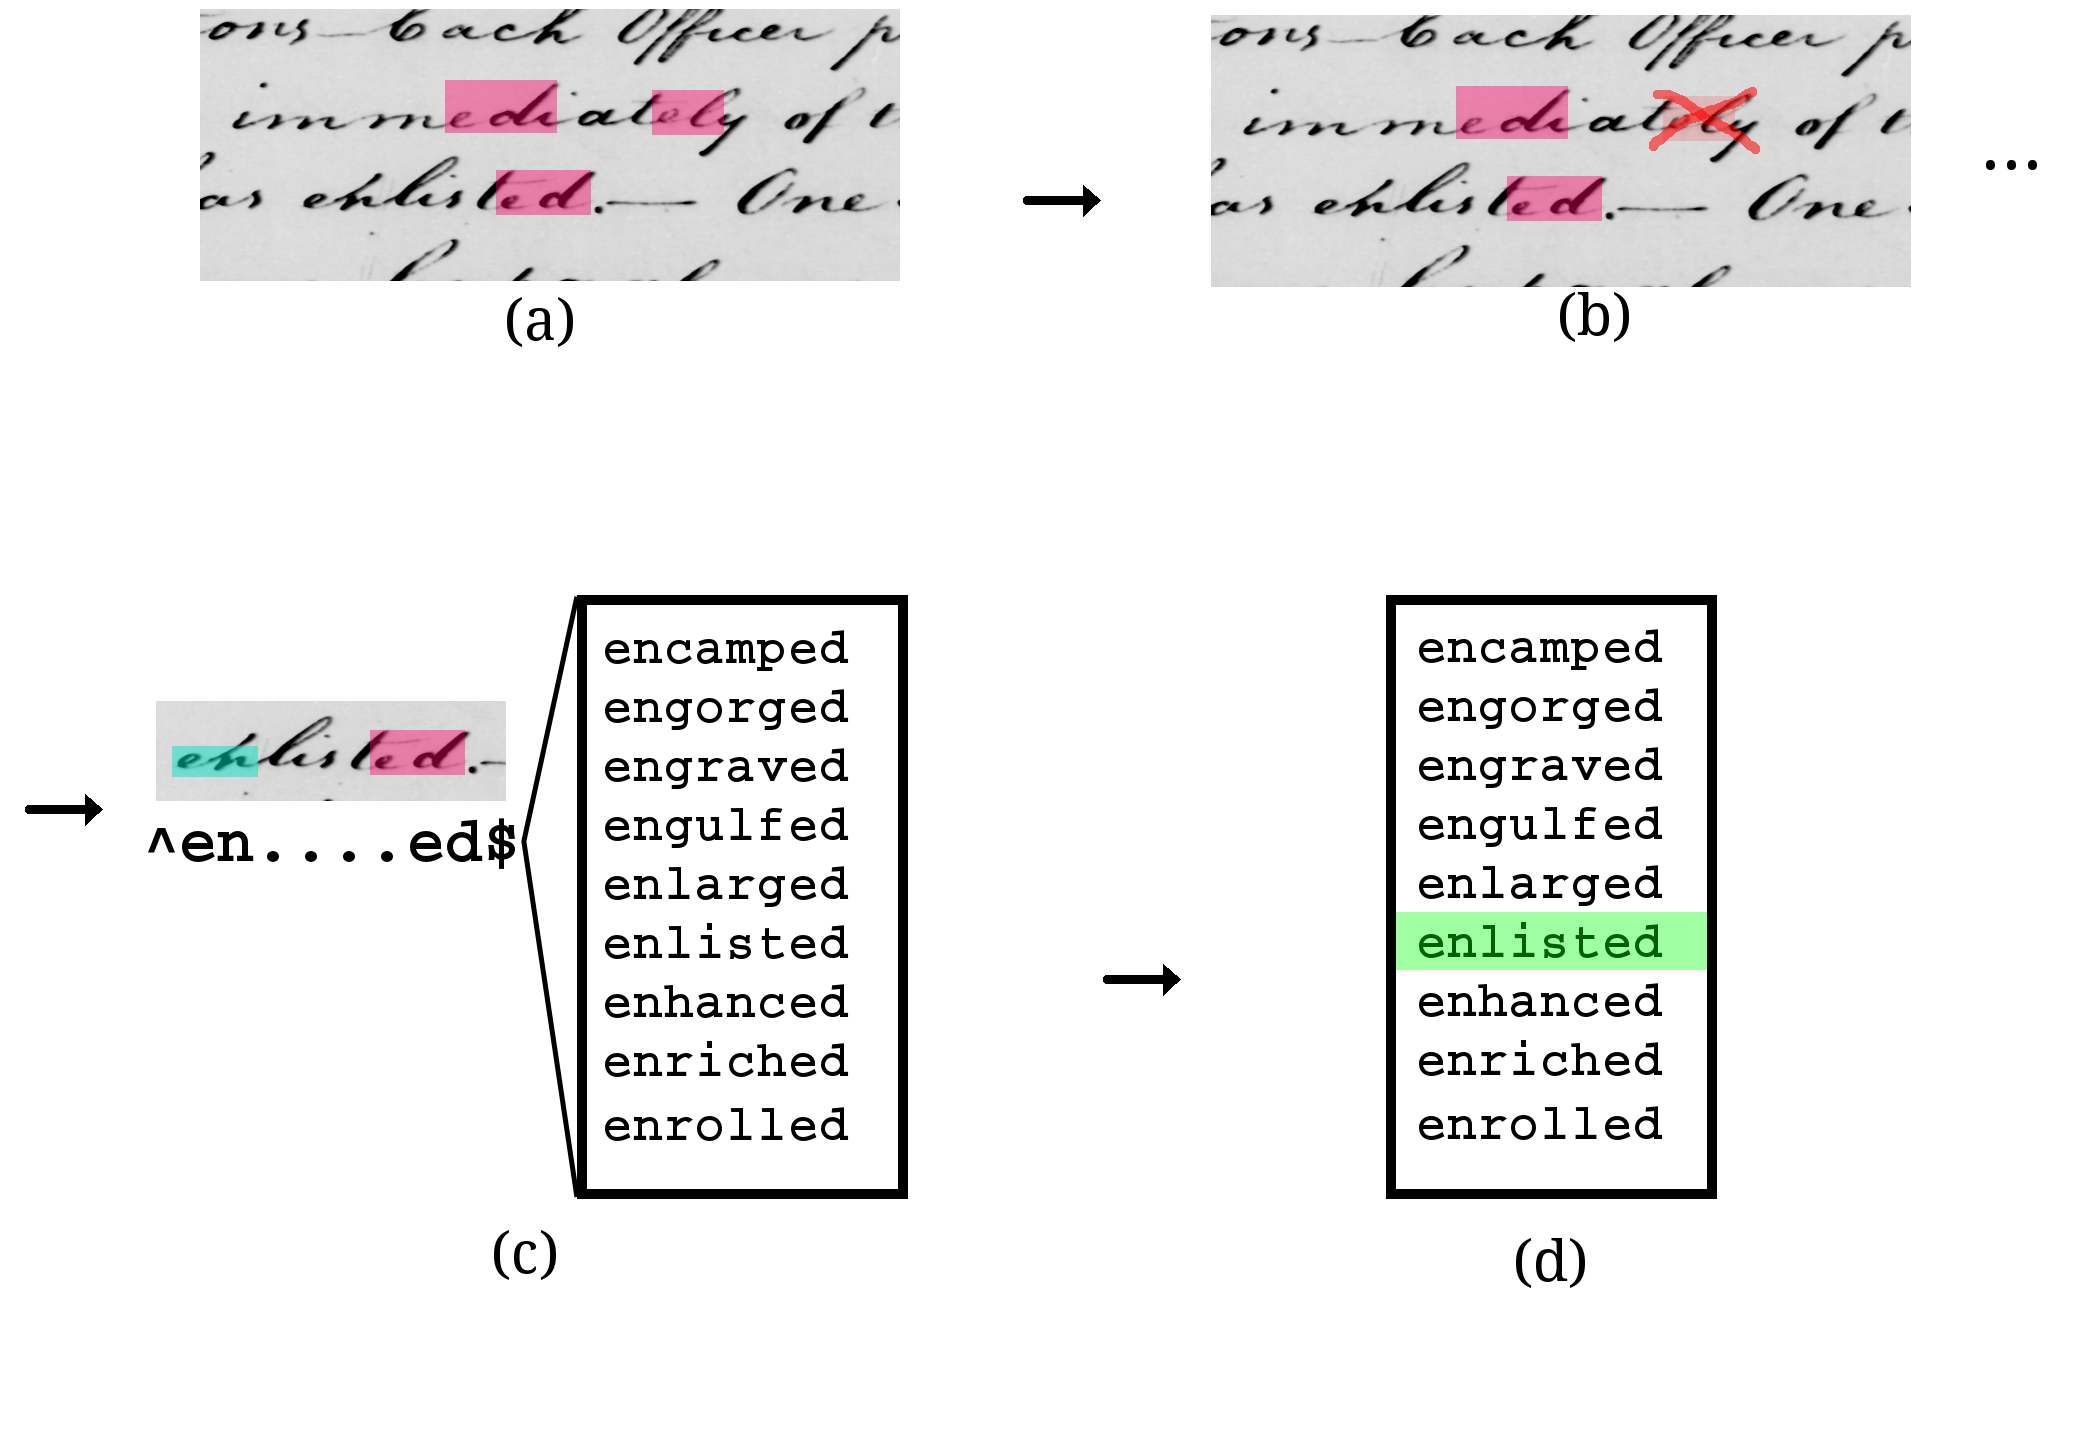
\includegraphics[width=.45\textwidth]{flow5}
    \caption{Work-flow of proposed CAT system. (a) N-grams are spotted by the system (``ed'' as an example here). (b) User removes false-positives (``el''). (c) After some iterations of n-gram spotting, a regular expression is generated (from ``en'' and ``ed'') and used to query the lexicon. (d) If 10 or less words are returned, present the list to a user to select the correct transcription (``enlisted'').}
    \label{fig:system_diagram}
\end{figure}

Let us examine the George Washington (GW) dataset\cite{GW} as an example of how effective this might be. If the 100 most frequent bigrams in the English language are spotted in the GW dataset with 49\% recall (i.e.~we actually spot only 49\% of the occurrences of each bigram), 53.6\% of the words in the corpus can be narrowed down to 10 or fewer possible transcriptions. This is assuming we can correctly guess the correct number of characters we haven't spotted in the words and using a 32,000 word lexicon. From this list of 10 or fewer words a user can easily select the correct transcription. More words can be transcribed as we use online learning to create new spotting queries; character n-grams that we missed will be spotted with subsequent queries. If subsequent queries also have 49\% recall, 75\% of the corpus can be transcribed with 250 spottings (i.e. going through the 100 bigrams 2.5 times). See Fig.~\ref{fig:fullSim} for the results of simulating this process. Preliminary results in spotting bigrams in the GW dataset have yielded a mean-average-precision greater than 60\%.

\begin{figure}
    \centering
    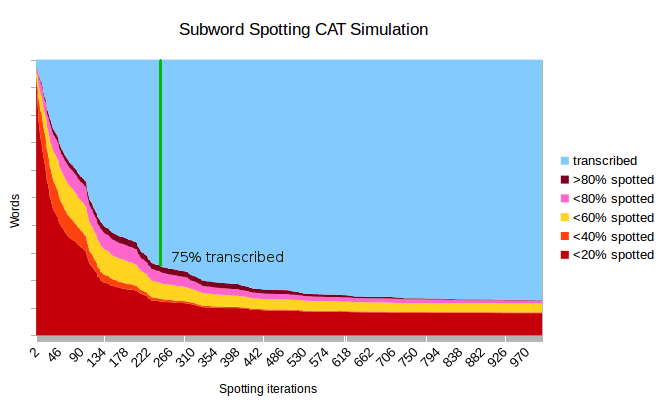
\includegraphics[width=.49\textwidth]{simulationGraph_line}
    \caption{Results of a simulation showing how much of the GW dataset can be transcribed after a given number of spotting iterations. The chart is drawn so one can observe the progress of spotting as well as transcription, each category (color) indicating the portion of words which have the given percent of their characters recognized by spottings (or indicating the portion of words transcribed).}
    \label{fig:fullSim}
\end{figure}

Like \cite{Neudecker2010}, the proposed system is flexible to all handwritten documents, is highly parallelizable, and has very simple user tasks. Of interest, small user tasks are ideal for casual mobile users. This can attract a larger audience of users, and this, combined with the parallelizable nature of the system, will make it ideal for crowdsourced transcription of historical handwritten documents.







% trigger a \newpage just before the given reference
% number - used to balance the columns on the last page
% adjust value as needed - may need to be readjusted if
% the document is modified later
%\IEEEtriggeratref{8}
% The "triggered" command can be changed if desired:
%\IEEEtriggercmd{\enlargethispage{-5in}}

% references section

% can use a bibliography generated by BibTeX as a .bbl file
% BibTeX documentation can be easily obtained at:
% http://mirror.ctan.org/biblio/bibtex/contrib/doc/
% The IEEEtran BibTeX style support page is at:
% http://www.michaelshell.org/tex/ieeetran/bibtex/
\bibliographystyle{IEEEtran}
% argument is your BibTeX string definitions and bibliography database(s)
\bibliography{IEEEabrv,bib}
%
%\bibliography{bib}
% <OR> manually copy in the resultant .bbl file
% set second argument of \begin to the number of references
% (used to reserve space for the reference number labels box)
%\begin{thebibliography}{1}

%\bibitem{IEEEhowto:kopka}
%H.~Kopka and P.~W. Daly, \emph{A Guide to \LaTeX}, 3rd~ed.\hskip 1em plus
%  0.5em minus 0.4em\relax Harlow, England: Addison-Wesley, 1999.

%\end{thebibliography}




% that's all folks
\end{document}


